\documentclass{amsbook}
\usepackage{graphicx} % Required for inserting images
\usepackage{float}
\usepackage[colorlinks=true,linkcolor=blue]{hyperref}
\usepackage{amssymb}
\usepackage{enumerate}
\usepackage{mathtools}
\usepackage{tikz}
\usepackage[answerdelayed]{exercise}
\usepackage{floatflt}
\usepackage{multicol}
\usepackage{subcaption}

\usepackage{tkz-euclide}

\usepackage{pgfplots}
\usetikzlibrary{trees}
\usepackage[backend=biber,style=alphabetic,sorting=ynt]{biblatex}
\addbibresource{calc.bib}

\setlength{\parindent}{0pt}
\setlength{\listparindent}{0pt}
\renewcommand{\ExerciseHeaderTitle}{\quad\ExerciseTitle}
\renewcommand{\AnswerHeader}{\medskip\centerline{\emph{\ExerciseName\ \ExerciseHeaderNB} \smallskip}}
\renewcommand{\ExerciseHeader}{\medskip\ExerciseHeaderDifficulty{\emph{\ExerciseName\ \ExerciseHeaderNB\ExerciseHeaderTitle} \newline}}
\renewcommand{\QuestionNB}{(\alph{Question})\ }

\tkzSetUpPoint[fill=black]
\begin{document}

\title{Geometry:\\
    \Large Form III}


\author{S. Chu}

\maketitle
\tableofcontents
\chapter*{Preface}
The following short booklet contains a collection of problems with solutions that roughly follow the topics typically covered in the Geometry course for Form III mathematics classes at Ethical Culture Fieldston School. The hope is to provide a book of problems of varying difficulty that will provide non-routine exercises as well as to record general themes and approaches to tackling these types of problems in general. Ideally these problems can be useful to all courses that cover these topics. Problems are roughly categorized by difficulty level and notated via *, **, or *** in increasing difficulty. We have adopted problems from memory, and from years of working with the material. The following references were consulted for problems as well as other considerations such as narrative structure in introducing various topics and thematic development of the material. \cite{mcirc}, \cite{aops}, \cite{hpn}, [more later].
\chapter{Pythagorean Theorem}
%%%%%%% template %%%%%%
%\begin{Exercise}[title= ,difficulty= ,label= ]
%\hfill \emph{solution} \refAnswer{}
%\end{Exercise}
%\begin{Answer}[ref={}]
%\end{Answer}

\begin{Exercise}[title={Two Rectangles and Two Squares}, difficulty=1, label=aa1]
	The squares in the diagram have sidelength one. What is the area of each rectangle?
	\begin{figure}[H]
	\centering
	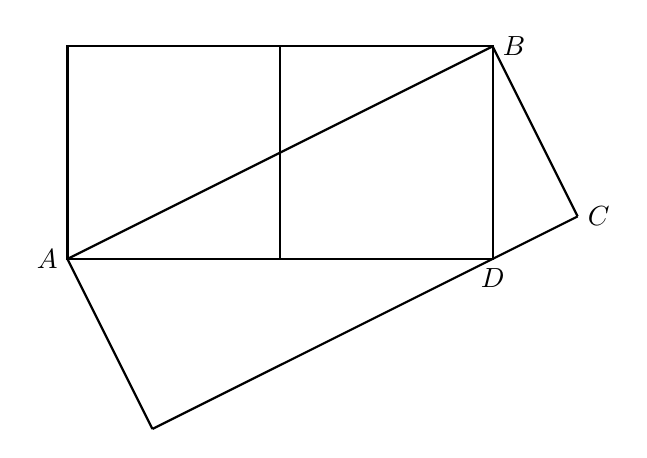
\begin{tikzpicture}[scale=.9]
		\draw[thick](0,0)--(0,3)--(3,3)--(3,0)--cycle;
		\draw[thick](3,3)--(6,3)--(6,0)--(3,0);
		\coordinate (A) at (0,0) node[below, left]{$A$};
		\coordinate (B) at (6,0);
		\coordinate (C) at (6,1.5);
		\coordinate (D) at (6,3);
		\coordinate (E) at (3,0);
		\draw(A)--(B) node[at end, below]{$D$};
		\draw[thick](A)--(D) node[at end,right]{$B$};
   		 \tkzDefLine[orthogonal=through A](D,A) \tkzGetPoint{a}
   		\tkzInterLC(A,a)(E,B) \tkzGetPoints{G}{H}
   		 %\draw(G)--(B);
   		 \draw[thick](H)--(B);
   		 \draw[thick](A)--(H);
   		 
   		 \tkzDefLine[orthogonal=through D](D,A) \tkzGetPoint{b}
   		 \tkzInterLC(D,b)(C,B) \tkzGetPoints{I}{J}
   		 \draw[thick](D)--(I) node[at end,right]{$C$};
   		 \draw[thick](B)--(I);
	\end{tikzpicture}
	\end{figure}
\hfill \emph{solution} \refAnswer{aa1}
\end{Exercise}

\begin{Answer}[ref={aa1}]
	The area of one rectangle is straightforward to calculate as you know each square has side length one so the dimensions of the rectangle made of these two squares is two by one, giving an area of 2. The second rectangle requires an application of the pythagorean theorem to get length of $\overline{AB}$, then use that $\Delta ABD \sim \Delta BDC$, which gives that $\dfrac{BC}{BD}=\dfrac{AD}{AB} \Rightarrow \dfrac{BC}{1}=\dfrac{2}{\sqrt{5}}$.  This gives the area of the second rectangle as $AB \cdot BC=\sqrt{5}\cdot \dfrac{2}{\sqrt{5}}=2$.
\end{Answer}

%%%%%%%%%%%%%%%%%%%%%%%%%%%%%%
\begin{Exercise}[title={A Circle Inscribed in a Right Triangle}, difficulty=1, label=aa6]
	Find the area of $\Delta ABC$, given that $DF=4$, $FB=36$.
	\begin{figure}[H]
		\centering
		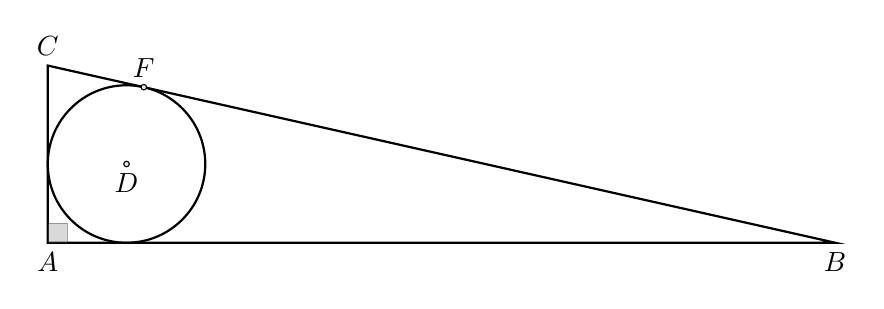
\begin{tikzpicture}
			\tkzDefPoints{0/0/A, 10/0/B, 0/2.25/C,1/1/D,1/0/E}
			\draw[thick](A)--(B)--(C)--cycle;
			\draw[thick](D) circle (1);
			\tkzLabelPoints(A,B,D)
			\tkzDefLine[mediator](B,C)
			\tkzDefPointBy[projection=onto B--C](D) \tkzGetPoint{F}
			\tkzDrawPoints(F,D)
			\tkzLabelPoints[above](C,F)
			\tkzMarkRightAngle[fill=gray, opacity=.3, size=0.25](B,A,C)
		\end{tikzpicture}
	\end{figure}

\hfill \emph{solution} \refAnswer{aa6}
\end{Exercise}

\begin{Answer}[ref={aa6}]
	The solution combines knowing that segments tangent to a circle and emanating from the same point are congruent with the pythagorean theorem. 
\end{Answer}
%%%%%%%%%%%%%%%%%%%%%

\begin{Exercise}[title={Five Inscribed Circles}, difficulty=2, label=aa5]
	The square has side length one. Find the length of the radius of the inscribed circles. All five circles have the same length radius.\\[.5cm]
	\begin{figure}[H]
	\centering
		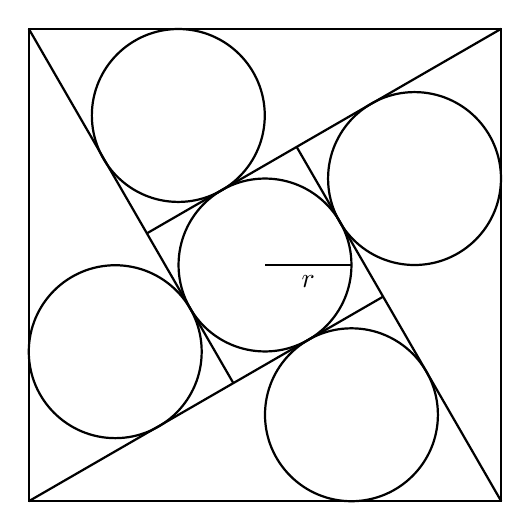
\begin{tikzpicture}[scale=3]
			\draw [thick](0,0)--(0,2)--(2,2)--(2,0)--cycle;
			\draw [thick](0,2)--++(0.866,-1.5);
			\draw [thick](0,0)--++(1.5,0.866);
			\draw[thick] (2,0)--++(-0.866,1.5);
			\draw[thick] (2,2)--++(-1.5,-0.866);
			\draw[thick] (1,1) circle (0.366);
			\draw[thick] (1.366,.366) circle(0.366);
			\draw[thick](.366,0.633) circle(0.366);
			\draw[thick](0.633, 1.633) circle(0.366);
			\draw[thick](1.633,1.366) circle(0.366);
			\draw[thick](1,1)--++(.366,0) node[midway, below]{$r$};
		\end{tikzpicture}
	\end{figure}
	\hfill \emph{solution} \refAnswer{aa5}
\end{Exercise}

\begin{Answer}[ref={aa5}]
	One solution to this problem involves recognizig that the area of the square is made up of a smaller square and four triangles whose areas can be expressed by the radius $r$. 
\end{Answer}
%%%%%%%%%%%

\begin{Exercise}[title={Distance From a Point to a Line}, difficulty =1, label =aa2]
	We can define the distance between a point $A$ and a line to be the the shortest distance between $A$ and any point on the line.
		\begin{enumerate}
			\item What is the distance between $A$ and a line $\ell$ if $A$ is on the line?\\
			\item If point $A$ is not on the line $\ell$, show that if point $B$ is at the intersection of the line $\ell$  and the line containing $A$ that is perpendicular to $\ell$, then $B$ is the closest point on $\ell$ to point $A$.
		\end{enumerate}
		\begin{figure}[H]
		\centering
		\begin{tikzpicture}[scale=1.5]
			\draw[draw opacity=0](0,0) grid (4,4);
			\draw[thick,<->](0,0)--(4,2) node[left, below]{$\ell$};
			\fill (2,2.5) circle[radius=1pt] node[left]{$A$};
		\end{tikzpicture}
		\end{figure}
		\vspace{1cm}
		\hfill \emph{solution} \refAnswer{aa2}
\end{Exercise}

\begin{Answer}[ref={aa2}]

\end{Answer}
%%%%%%%%%%%%
\begin{Exercise}[title={Lines Tangent to a Circle}, difficulty=1, label=aa3]
	A line is tangent to a circle if it meets the circle at one and only one point. In the figure below the line containing $A$ and $B$ meets the circle centered at point $X$ at point $B$. Prove that $\overline{XB}$ is perpendicular to the line. Hint: Start by assuming they are not perpendicular.\\
	
	\vspace{.5cm}
	\hfill \emph{solution} \refAnswer{aa3}
\end{Exercise}

\begin{Answer}[ref={aa3}]

\end{Answer}

%%%%%%%%%%%%%%%%%
\begin{Exercise}[title={A Surprising Ratio}, difficulty=2, label=aa4]
	Find the ratio of the length $R$ to the length $d$. All circles are tangent to one another.\\
		\begin{figure}[H]
		\centering
		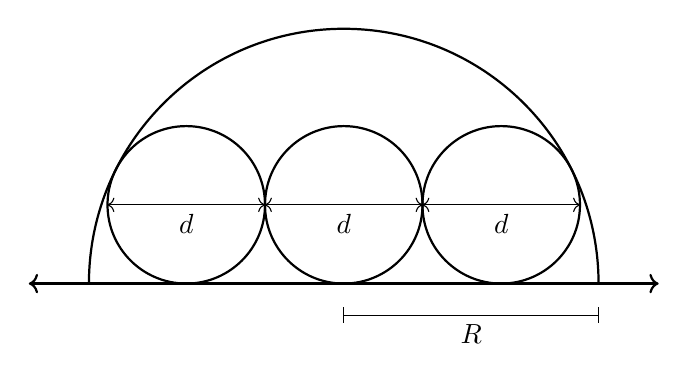
\begin{tikzpicture}[scale=2]
			\def\tick{0.05} %define the height of tick marks
				\draw[thick] (1.618,0) arc (0:180:1.618); % Draw a semicircle with radius 1.61
				\draw [thick](0,.5) circle(0.5);
				\draw[thick](1,.5) circle(0.5);
				\draw[thick](-1,.5) circle(0.5);
				\draw[<->, thick](-2,0) -- (2,0);
				\coordinate(A) at (0,-.2);
				\coordinate(B) at (1.618,-.2);
				\draw(A) --(B) node[midway, below]{$R$};
				\draw(0,-.2+\tick)-- ++(0,-2*\tick);
				\draw(1.618, -.2+\tick)--++(0, -2*\tick);
				\coordinate(C) at (-1.5,.5);
				\coordinate(D) at (-.5, .5);
				\coordinate(E) at (.5, .5);
				\coordinate(F) at (1.5, .5);
				\draw[<->](C)--(D) node[midway, below]{$d$};
				\draw[<->](D)--(E) node[midway, below]{$d$};
				\draw[<->](E)--(F) node[midway, below]{$d$};
			\end{tikzpicture}
			\end{figure}
			\hfill \emph{solution} \refAnswer{aa4}
			
\end{Exercise}
	
\begin{Answer}[ref={aa4}]


\end{Answer}

\chapter{Objects of Geometry}

\begin{Exercise}[title={A few well known sets}, difficulty=0, label=1a1]
Let $\mathbb{N}=\{1,2,3,4,\ldots\}$. These are the natural numbers or counting numbers. $\mathbb{Z}=\{\ldots, -2, -1, 0, 1, 2,3,\ldots\}$ is the set of integers. $\mathbb{Q}=\{p/q \, \big| \, p, q \in \mathbb{Z}\}$ is the set of rational numbers. $\mathbb{R}$ refers to the set of real numbers. $\mathbb{C}$ refers to the set of complex numbers.
    \Question Fill in the blank with $\subset$ or $\supset$. \quad $\mathbb{Z} \, \makebox[1em]{\hrulefill}\, \mathbb{N}$
    \Question Fill in the blank with $\subset$ or $\supset$. \quad $\mathbb{R} \, \makebox[1em]{\hrulefill} \, \mathbb{Q}$
    \Question Fill in the blank with $\subset$ or $\supset$. \quad $\mathbb{N} \, \makebox[1em]{\hrulefill} \, \mathbb{Q}$
    
    \hfill \emph{solution} \refAnswer{1a1}
\end{Exercise}

\begin{Answer}[ref={1a1}]
    The expression $A \subset B$ is read, the set $A$ is contained in the set $B$. Whereas the expression $A \supset B$ is read the set $A$ contains the set $B$.
    \begin{enumerate}
        \item $\mathbb{Z}\supset \mathbb{N}$
        \item $\mathbb{R}\supset \mathbb{Q}$
        \item $\mathbb{N} \subset \mathbb{Q}$
    \end{enumerate}
\end{Answer}
%%



%%%%%%%%%%%%%%%%%%%%%%%%%%%%%%%%%%%%%%%%
\chapter{Lines}
This chapter reinforces content about lines from an Algebra 1 course. We will deepen this understanding by combining the algebra of lines with the ability to calculate lengths and find midpoints. We will also introduce the idea of parameterized lines in preparation for an algebraic description of lines and planes in 3-space. In parallel to these analytic aspects of lines we will talk about what we can determine about lines in the absence of coordinates, developing the idea of parallel and perpendicular along with typical theorems involving two lines and a transversal. This discussion leads naturally to the sum of the interior angles of a triangle and theorems around interior and exterior angles of polygons in general. 

\section{Lines with Coordinates}
\begin{Exercise}[title={A point $(x,y)$} ,difficulty=0 ,label=3a1 ]
Given a point $A(3,-1)$, there are many lines that include this point.
	\begin{enumerate}
		\item Give the equation of the horizontal line that includes $A$.
		\item Give the equation of the vertical line that includes $A$.
		\item Give the equation of the line that includes $A$ and has slope $m=-1$.
		\item How many different lines pass through the point $A$? Construct an argument to convince others you are right.
	\end{enumerate}
\hfill \emph{solution} \refAnswer{3a1}
\end{Exercise}
\begin{Answer}[ref={3a1}]
 	\begin{enumerate}
 		\item $y=-1$
 		\item $x=3$
 		\item $x+y=2$
 		\item There are many approaches to arguing why there are an infinite number of lines passing through $A$. One possibility is to associate $y=-1$ with $0^\circ$ and $x=3$ with $90^\circ$ then every angle between $0^\circ$ and $90^\circ$ can be associated with a line through $A$ and since there are an infinite number of numbers then there are an infinite number of lines as well.
 	\end{enumerate}
\end{Answer}

\begin{Exercise}[title={Two Points} ,difficulty=0 ,label=3a2 ]
	Let $A(3,-1)$ and $B(-5,3)$. 
		\begin{enumerate}
			\item Give the equation of the line that contains $\overline{AB}$ in point slope form.
			\item Give the equation of the line that contains $\overline{AB}$ in slope intercept form.
			\item Give the equation of the line that contains $\overline{AB}$ in standard form $ax+by=c$ where $a,b,c$ are integers.
		\end{enumerate}
\hfill \emph{solution} \refAnswer{3a2}
\end{Exercise}
\begin{Answer}[ref={3a2}]
\end{Answer}

\section{Vectors}

\section{Parametric Lines}

\section{Lines without Coordinates}


\chapter{Angles and Polygons}

\section{Triangles}

\section{Polygons}


\chapter{In Depth with Triangles}

\section{Congruent Triangles}

\section{Points of Concurrency}


\chapter{Quadrilaterals}
\begin{Exercise}[title={Interesting Family of Quadrilaterals},difficulty=2 ,label=6a1 ]
	Find all the ways to arrange 4 distinct points only two different distances occur between any two points.
	\hfill \emph{solution} \refAnswer{6a1}
\end{Exercise}
\begin{Answer}[ref={6a1}]

\end{Answer}


\chapter{More Coordinate Geometry}

\chapter{Isometries}

\section{Translations}

\section{Rotations}

\section{Reflections}

\section{Glide Reflections}

\section{Composition of Isometries}

\section{Symmetries}
\begin{Exercise}[title={Layer Cake} ,difficulty=2 , label=8f1 ]
	You have a rectangular layer cake, that has an arbitrarily placed rectangular hole taken out of it. Give a procedure that will always work for cutting this cake with one straight cut into two pieces of equal volume so that each piece has all layer of the cake. 
	\hfill \emph{solution} \refAnswer{8f1}
\end{Exercise}
\begin{Answer}[ref={8f1}]
	The essential piece of knowledge for this problem is that the rectangle has point symmetry. Thus any line through the center of the object, the point about which the figure has point symmetry, will cut the rectangle into two pieces of equal area. This can be proven using the idea that isometries preserved length and area. 
\end{Answer}


\chapter{Similarity}
\begin{Exercise}[title={Almost the same}, difficulty=2, label=9a1]
There are two non-congruent triangles. These two triangles have 5 out of their 6 components (3 angles and 3 sides) congruent. The larger area triangle's longest side has length 32. The smaller area triangle's shortest side has a side length of 8. What is the product of the smaller triangle's side lengths?
\hfill \emph{solution} \refAnswer{9a1}
\end{Exercise}

\begin{Answer}[ref={9a1}]
If 5 out of 6 of the two triangles' components are congurent then either the set of sides has the same lengths or the set of angles has the same measure. If the set of sides have the same length then the triangles must be congruent, which contradicts the given situation. Thus, the triangles angles are congurent and they are similar. The smallest side of each triangle cannot be 8 otherwise the similarity ratio would be 1:1 and the triangles would be congruent. Thus, listing the ratio of sides from smaller triangle to larger triangle, we have that $\dfrac{8}{x}=\dfrac{x}{y}=\dfrac{y}{32}$. The smaller triangle has side lengths $\{8,x,y\}$ and the larger triangle has side length $\{x,y,32\}$. From these we get the equations:

\end{Answer}

\begin{Exercise}[title={Triangles in a Semicircle}, difficulty=3, label=9a2]
There are 3 chords in a semicircle  of length 3, 3, and 7 such that the chords connect end to end with the outer chords having endpoints at the ends of the diameter of the semicircle. Find the radius of the circle. 
\end{Exercise}

\begin{Answer}[ref={9a2}]

\end{Answer}

\chapter{Trigonometry}
\begin{Exercise}[title={Regular Polygons Inscribed in a Circle} ,difficulty=2 ,label=10a1 ]
	Find the radius of the circle below, if the three congruent squares have a side length of four, and the regular triangle shares sides with each of the three squares.
	\begin{figure}[H]
	\centering
	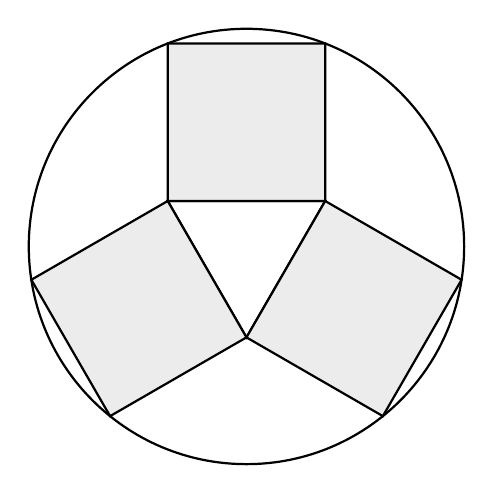
\begin{tikzpicture}[scale=2]
		\tkzDefPoints{0/0/A, 0.5/.2887/B}
		\draw[thick](A)circle(1.3823);
		\tkzDefRegPolygon[center, sides=3](A,B)
		\draw[thick](P1)--(P2)--(P3)--cycle;
		\tkzDefRegPolygon[side, sides=4,name=Q](P2,P1)
		\tkzFillPolygon[gray!15](Q1,Q2,Q3,Q4)
		\draw[thick](Q2)--(Q3)--(Q4)--(Q1)--cycle;
		\tkzDefRegPolygon[side,sides=4,name=R](P3,P2)
		\tkzFillPolygon[gray!15](R1,R2,R3,R4)
		\draw[thick](R2)--(R3)--(R4)--(R1)--cycle;
		\tkzDefRegPolygon[side,sides=4,name=S](P1,P3)
		\tkzFillPolygon[gray!15](S1,S2,S3,S4)
		\draw[thick](S2)--(S3)--(S4)--(S1)--cycle;
	\end{tikzpicture}
	\end{figure}	
	
\hfill \emph{solution} \refAnswer{10a1}
\end{Exercise}
\begin{Answer}[ref={10a1}]
\end{Answer}


\chapter{Area}

\chapter{Volume and 3 space}


\chapter{Circles}


%End of problems of the book.

\chapter{Answers}
\shipoutAnswer

\printbibliography
\end{document}
